\documentclass[a4paper,12pt]{article}
% Math essential packages
\usepackage{latexsym, mathtools}
\usepackage{amsmath, amssymb, amsfonts, amsthm, amsxtra}
\usepackage[nomathsymbols]{polski}
\usepackage{amscd, tikz-cd}
\usepackage[skip=10pt, indent=0pt]{parskip}
\usepackage[a4paper, left=30mm, right=30mm, top=25mm, bottom=25mm]{geometry}
\usepackage{graphicx, float}
\usepackage{xcolor}
\usepackage[most,many,breakable]{tcolorbox}
\usepackage{relsize}
\usepackage{fancyhdr}
\usepackage{url}
\usepackage[colorlinks=true,citecolor=blue,urlcolor=blue,linkcolor=blue,pdfpagemode=UseNone]{hyperref}

\usepackage[framemethod=TikZ]{mdframed}
\usepackage{thmtools}

\usepackage{XCharter}

\title{Regresja liniowa - skrypt}
\author{Zachariasz Jażdżewski}

\begin{document}
\maketitle

%----Proper document------------------------------------------------------------

\section{Czym jest dopasowanie prostej}
Załóżmy, że jesteśmy badaczami zajmującymi się analizą wzrostu roślin w różnych warunkach środowiskowych. Przez kilka miesięcy zbieraliśmy dane dotyczące wysokości roślin oraz ilości dostarczanego im światła słonecznego w różnych dniach. 

\begin{center}
	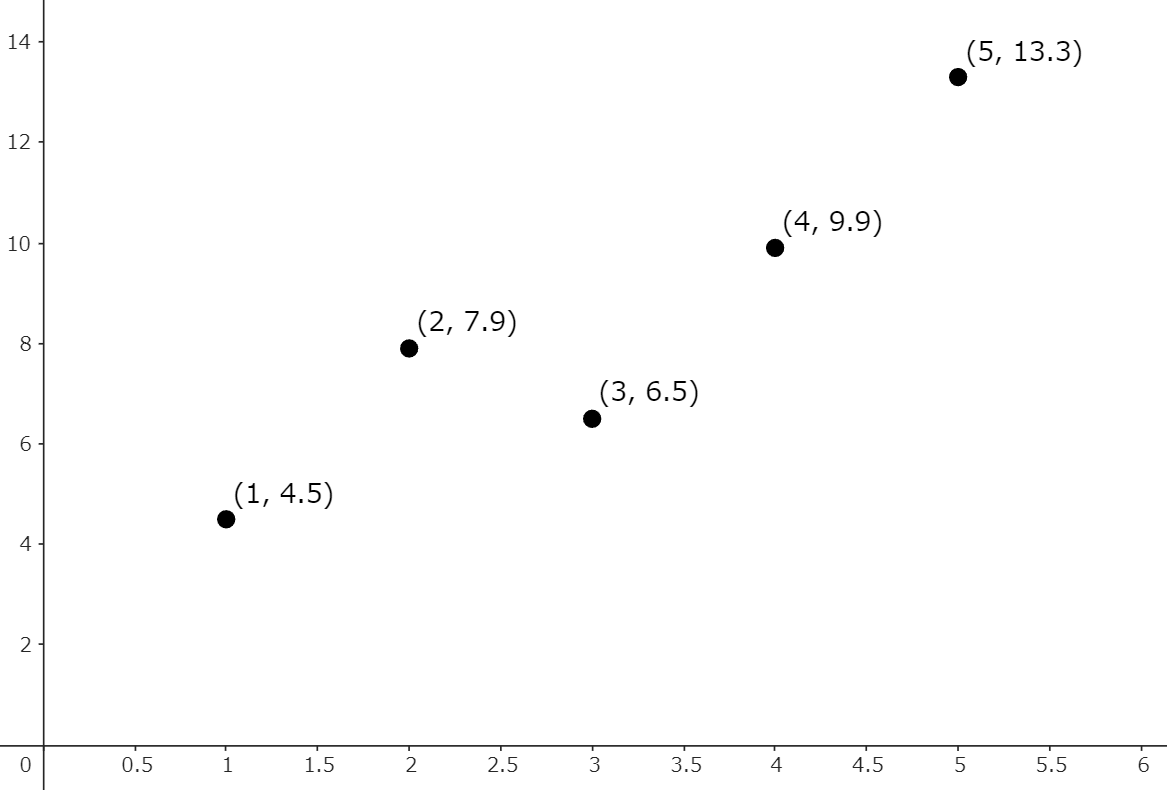
\includegraphics[width=0.7\textwidth]{Figures/figure-1.png}
\end{center}

\begin{table}[h]
    \centering
    \begin{tabular}{|c|c|c|c|c|c|}
        \hline
        \textbf{Światło słoneczne (kiloluks)} & 1 & 2 & 3 & 4 & 5 \\
		\hline
        \textbf{Wzrost roślin (cm)} & 4.5 & 7.9 & 6.5 & 9.9 & 13.3 \\
        \hline
    \end{tabular}
\end{table}

Po przejrzeniu tych danych i rozrysowaniu ich na wykresie zauważyliśmy pewne trendy, które sugerują, że istnieje związek między ilością światła słonecznego a wzrostem roślin. W związku z tym zastanawiamy się, w jaki sposób możemy stworzyć model, który pozwoliłby nam przewidzieć wzrost roślin na podstawie dostarczanego im światła słonecznego.

Metodę znajdowania takiego modelu nazywa się regresją liniową. Regresja liniowa polega na badaniu zależności między zmiennymi; w najprostszej formie jest to technika modelowania zależności między tylko dwiema zmiennymi (jak na przykład nasze dane rozłożone w czasie). My zajmiemy się prostym przykładem regresji liniowej, jakim jest dopasowanie prostej do zestawu danych, wykorzystując metodę najmniejszych kwadratów.

\newpage

\section{Metoda najmniejszych kwadratów i najlepsze rozwiązanie układu równań}
Przedstawimy twierdzenie, które bardzo przyda się przy omawianiu zagadnienia regresji liniowej.
\begin{theorem}
	Zbiór najlepszych rozwiązań układu równań \(Ax = b\) jest identyczny ze zbiorem rozwiązań układu \(A^T Ax = A^T b\). 
	\[
		Ax = b \iff A^T Ax = A^T b
	\]
\end{theorem}
\begin{note}
	Taki sposób wyznaczania najlepszego rozwiązania układu równań \\ liniowych nazywamy \emph{metodą najmniejszych kwadratów}, a sam układ równań \\ \(A^T Ax = A^T b\) nazywamy \emph{normalnym}
\end{note}

\section{Dopasowanie prostej}
Niech \((x_1, y_2), (x_2, y_2), \dots , (x_{n}, y_{n})\) będą punktami z płaszczyzny \(\R^2\) takimi, że nie wszystkie liczby \(x_1,x_2, \dots , x_{n}\) są równe. Wyznaczymy prostą \(y = ax + b\), która najlepiej pasuje do danych punktów. Jej współczynniki \(a\) i \(b\) dobieramy w taki sposób, aby suma
\[
	\sum_{i=1}^{n} (ax_{i} + b - y_{i})^2
\]    
w której \(|ax_{i} + b - y_{i}|\) jest odległością pomiędzy punktami \((x_i, y_i)\) i \((x_i, ax_i + b)\) była najmniejsza z możliwych. 

Suma ta jest najmniejsza wtedy i tylko wtedy, gdy \((a,b)\) jest \emph{najlepszym rozwiązaniem} układu równań liniowych:
\[
	\begin{dcases}
		ax_1 + b = y_1 \\
		ax_2 + b = y_2 \\
		\qquad \vdots \\
		ax_n + b = y_n
	\end{dcases}
\]

Taki układ możemy zapisać w postaci macierzowej jako \(Ax = b\), gdzie
\[
	A = 
	\begin{bmatrix}
		x_1 & 1 \\
		x_2 & 1 \\
		\vdots & \vdots \\
		x_n & 1
	\end{bmatrix},
	\quad
	x = 
	\begin{bmatrix}
		a \\
		b
	\end{bmatrix},
	\quad
	b = 
	\begin{bmatrix}
		y_1 \\
		y_2 \\
		\vdots \\
		y_n
	\end{bmatrix}
\]

\newpage

Korzystając z poznanego twierdzenia, najlepsze rozwiązanie tego układu wyznaczamy za pomocą \emph{normalnego układu równań} \(A^T A x = A^T b\):
\[
	A^T A = \begin{bmatrix}
		x_1 & \dots & x_n \\
		1 & \dots & 1
	\end{bmatrix}
	\begin{bmatrix}
		x_1 & 1 \\
		x_2 & 1 \\
		\vdots & \vdots \\
		x_n & 1
	\end{bmatrix}
	=
	\begin{bmatrix}
		\sum_{i=1}^{n} x_i^2 &  \sum_{i=1}^{n} x_i \\
		\sum_{i=1}^{n} x_i & n
	\end{bmatrix}
\] 
\[
	A^T b = 
	\begin{bmatrix}
		x_1 & \dots & x_n \\
		1 & \dots & 1  \\
	\end{bmatrix}
	\begin{bmatrix}
		 y_1 \\
		 y_2 \\
		 \vdots \\
		 y_n \\
	\end{bmatrix}
	=
	\begin{bmatrix}
		 \sum_{i=1}^{n} x_i y_i \\
		 \sum_{i=1}^{n} y_i  \\
	\end{bmatrix}
\]

Możemy zauważyć, że wyznacznik macierzy \(A^T A\) jest równy
\[
	\sum_{1 \leq i < j \leq n} (x_{i} - x_{j})^2 
\]
Zatem ostateczna suma jest niezerowa tylko wtedy, gdy nie wszystkie liczby \(x_1, \dots , x_n\) są równe. Stąd też układ \(A^T Ax\) = \(A^T b\) ma dokładnie jedno rozwiązanie (a co za tym idzie układ \(Ax = b\) ma dokładnie jedno \emph{najlepsze} rozwiązanie), jeśli tylko nie wszystkie liczby \(x_1, \dots , x_n\) są równe.

\section{Jak to się liczy}
\subsection{Prosty przykład}
Wyznaczymy najlepszą liniową zależność \(y = ax + b\) między współrzędnymi \(x_i\) i \(y_i\) punktów \((0,0), (3,3), (6,4), (9,4)\) i \((12,7)\). 
\begin{center}
	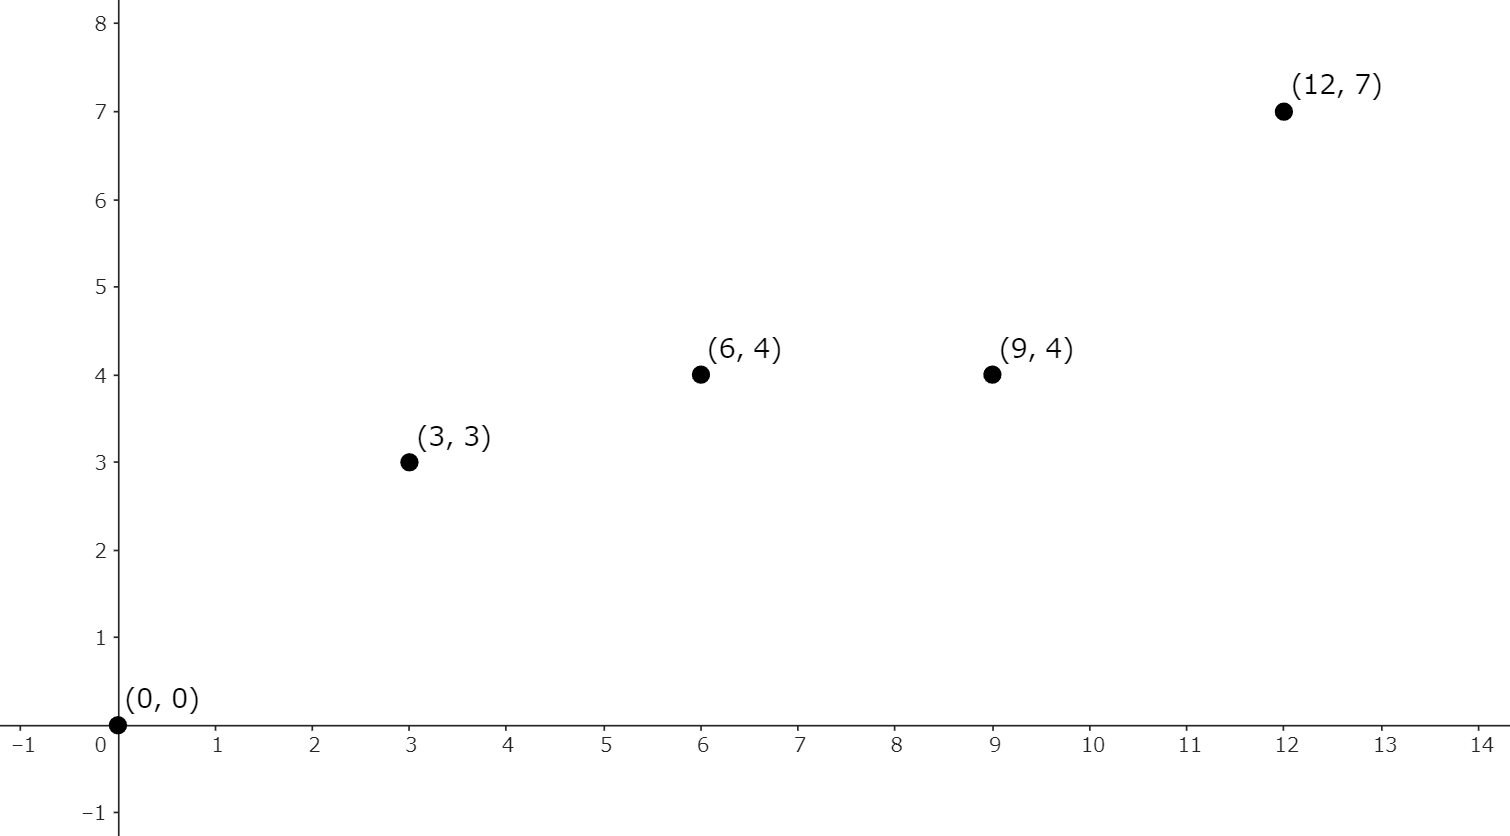
\includegraphics[width=0.9\textwidth]{Figures/figure-2.png}
\end{center} 

\newpage

Szukane współczynniki \(a\) i \(b\) są najlepszym rozwiązaniem układu równań liniowych \(Ax = b\), gdzie
\[
	A = 
	\begin{bmatrix}
		0 &  1 \\
		3 &  1 \\
		6 &  1 \\
		9 &  1 \\
		12 &  1 \\
	\end{bmatrix}
	,\quad
	x = 
	\begin{bmatrix}
		 a \\
		 b \\
	\end{bmatrix}
	,\quad
	b = 
	\begin{bmatrix}
		 0 \\
		 3 \\
		 4 \\
		 4 \\
		 7 \\
	\end{bmatrix}
\]

Za pomocą poznanej metody najmniejszych kwadratów, aby rozwiązać takie równanie, musimy rozwiązać normalny układ równań \(A^T Ax = A^T b\). Mamy zatem
\[
	A^T A = 
	\begin{bmatrix}
		0 & 3 & 6 & 9 &  12 \\
		1 & 1 & 1 & 1 &  1 \\
	\end{bmatrix}
	\begin{bmatrix}
		0 &  1 \\
		3 &  1 \\
		6 &  1 \\
		9 &  1 \\
		12 &  1 \\
	\end{bmatrix}
	=
	\begin{bmatrix}
		270 &  30 \\
		30 &  5 \\
	\end{bmatrix}
\]
\[
	A^T b = 
	\begin{bmatrix}
		0 & 3 & 6 & 9 &  12 \\
		1 & 1 & 1 & 1 &  1 \\
	\end{bmatrix}
	\begin{bmatrix}
		 0 \\
		 3 \\
		 4 \\
		 4 \\
		 7 \\
	\end{bmatrix}
	=
	\begin{bmatrix}
		 158 \\
		 18 \\
	\end{bmatrix}
\]

Rozwiązujemy zatem układ równań
\begin{gather*}
	A^T Ax = A^T b \\
	(A^T A)^{-1} (A^T A)x = (A^T A)^{-1} (A^Tb) \\
	x = (A^T A)^{-1} (A^Tb)
\end{gather*}
\[
	x = 
	\begin{bmatrix}
		270 &  30 \\
		30 &  5 \\
	\end{bmatrix}^{-1} 
	\begin{bmatrix}
		158 \\
		18 \\
   \end{bmatrix}
   =
   \begin{bmatrix}
	 \sfrac{5}{9} \\
	 \sfrac{4}{15} \\
   \end{bmatrix}
\]

Otrzymaliśmy zatem, że prosta \(y = \frac{5}{9}x + \frac{4}{15}\) jest najlepszą liniową zależnością pomiędzy współrzędnymi punktów \((0,0), (3,3), (6,4), (9,4)\) i \((12,7)\).  

\begin{center}
	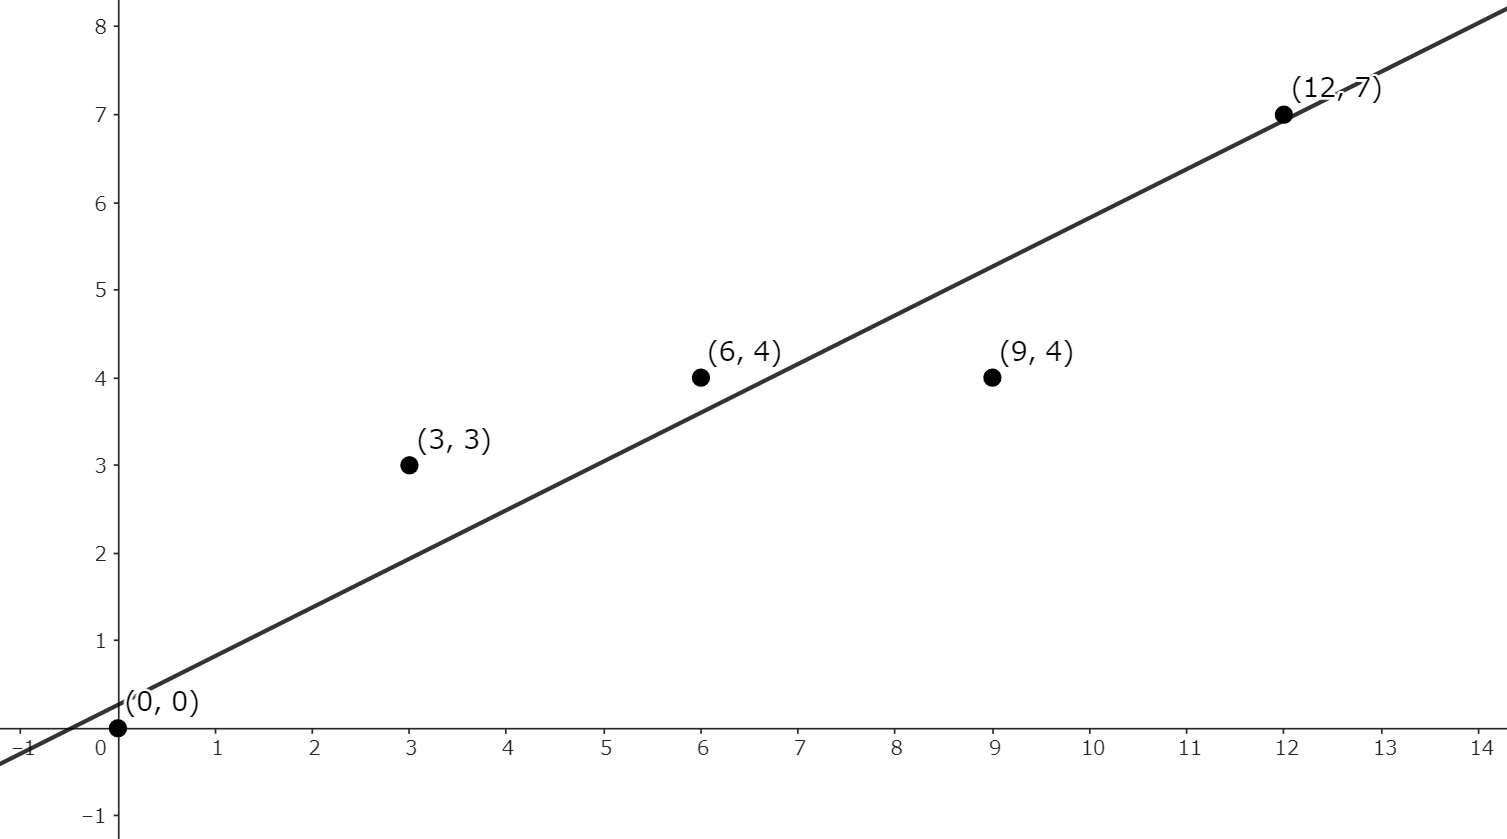
\includegraphics[width=0.9\textwidth]{Figures/figure-3.png}
\end{center}

\subsection{Zastosowanie}
Skoro poznaliśmy już narzędzie dopasowania prostej, spróbujmy je wykorzystać przy problemie ze wstępu. Znajdźmy prostą która będzie najlepiej dopasowana do danych o wzroście roślin.

Przypomnijmy, badaliśmy wzrost roślin przy różnych ilościach światła. Dane mamy podane w tabeli:
\begin{table}[h]
    \centering
    \begin{tabular}{|c|c|c|c|c|c|}
        \hline
        \textbf{Światło słoneczne (kiloluks)} & 1 & 2 & 3 & 4 & 5 \\
		\hline
        \textbf{Wzrost roślin (cm)} & 4.5 & 7.9 & 6.5 & 9.9 & 13.3 \\
        \hline
    \end{tabular}
\end{table}

Mamy zatem układ równań \(Ax = b\), gdzie: 
\[
	A = 
	\begin{bmatrix}
		1 &  1 \\
		2 &  1 \\
		3 &  1 \\
		4 &  1 \\
		5 &  1 \\
	\end{bmatrix},
	\quad
	x = 
	\begin{bmatrix}
		 a \\
		 b \\
	\end{bmatrix},
	\quad
	b = 
	\begin{bmatrix}
		 4.5 \\
		 7.9 \\
		 6.5 \\
		 9.9 \\
		 13.3 \\
	\end{bmatrix}
\]

Konstruujemy \emph{układ normalny} \(A^T Ax = A^T b\). Policzmy macierze \(A^T A\) i \(A^T b\):
\[
	A^T A = 
	\begin{bmatrix}
		1 & 2 & 3 & 4 &  5 \\
		1 & 1 & 1 & 1 &  1 \\
	\end{bmatrix}
	\begin{bmatrix}
		1 &  1 \\
		2 &  1 \\
		3 &  1 \\
		4 &  1 \\
		5 &  1 \\
	\end{bmatrix}
	=
	\begin{bmatrix}
		55 &  15 \\
		15 &  5 \\
	\end{bmatrix}
\]
\[
	A^T b = 
	\begin{bmatrix}
		1 & 2 & 3 & 4 &  5 \\
		1 & 1 & 1 & 1 &  1 \\
	\end{bmatrix}
	\begin{bmatrix}
		4.5 \\
		7.9 \\
		6.5 \\
		9.9 \\
		13.3 \\
   \end{bmatrix}
   = 
   \begin{bmatrix}
	 145.9 \\
	 42.1 \\
   \end{bmatrix}
\]

Mając macierze \(A^T A\) i \(A^T b\) wystarczy rozwiązać równanie macierzowe. Tym razem skorzystamy z metody eliminacji Gaussa.
\[
	[\,A\,|\,b\,]
	\quad
	\overset{\text{operacje elementarne}}{\xrightarrow{\hspace{3cm}}}
	\quad
	[\,I\,|\,x\,]
\]

\newpage

Podstawiając wartości otrzymujemy:
\[
	\begin{bmatrix}
		55 & 15 & \bigm| & 145.9 \\
		15 & 5 & \bigm| & 42.1
	\end{bmatrix}
	\sim
	\begin{bmatrix}
		1 & \frac{3}{11} & \bigm| & \frac{1459}{550} \\
		15 & 5 & \bigm| & \frac{421}{10} \\
	\end{bmatrix}
	\sim
	\begin{bmatrix}
		1 & \frac{3}{11} & \bigm| & \frac{1459}{550} \\
		0 & \frac{10}{11} & \bigm| & \frac{127}{55}  \\
	\end{bmatrix}
	\sim
\]
\[
	\begin{bmatrix}
		1 & \frac{3}{11} & \bigm| & \frac{1459}{550} \\
		0 & 1 & \bigm| & \frac{125}{50} \\
	\end{bmatrix}
	\sim
	\begin{bmatrix}
		1 & 0 & \bigm| & \frac{49}{25} \\
		0 & 1 & \bigm| & \frac{127}{50} \\
	\end{bmatrix}
	=
	\begin{bmatrix}
		1 & 0 & \bigm| & 1.96 \\
		0 & 1 & \bigm| & 2.54 \\
	\end{bmatrix}
\]

Rozwiązaniem naszego układu równań jest więc \(a = 1.96\) i \(b = 2.54\), zatem prosta \(y = 1.96x + 2.54\) jest najlepszą liniową zależnością między naszymi punktami. Narysujmy ją zatem na wykresie.

\begin{center}
	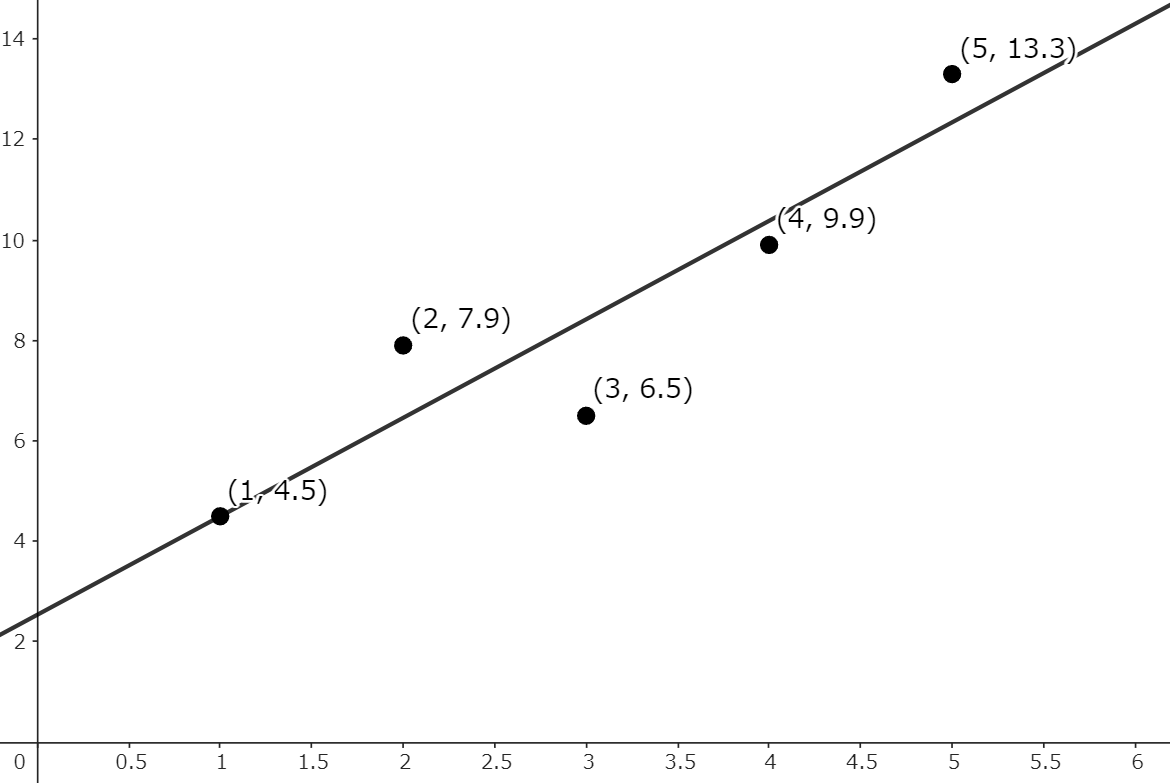
\includegraphics[width=0.75\textwidth]{Figures/figure-4.png}
\end{center}

\section{Wnioski}
Jak zobaczyliśmy, regresja liniowa jest bardzo przydatnym narzędziem używanym na codzień w przeróżnych dziedzinach nauki, szczególnie gdy mamy potrzebę analizy i interpretacji danych. Dzięki niemu możemy skutecznie modelować zależności między zmiennymi oraz prognozować przyszłe zachowania. Przy wyższym poziomie zaawansowania możemy nawet dopasowywać różnorakie funkcje wielomianowe co pozwala na jeszcze bardziej precyzyjne predykcje.  


%-------------------------------------------------------------------------------

\end{document}
